\documentclass{article} % For LaTeX2e
\usepackage{nips_adapted,times}
\usepackage{hyperref}
\usepackage{url}
\usepackage{graphicx}
\usepackage{subfig}

\title{Project Report: Analysis of Hillary Clinton E-mails}


\author{
Debojyoti Dey \\
15511264 \\
\And
Nimisha Agarwal \\
15511267 \\
}

% The \author macro works with any number of authors. There are two commands
% used to separate the names and addresses of multiple authors: \And and \AND.
%
% Using \And between authors leaves it to \LaTeX{} to determine where to break
% the lines. Using \AND forces a linebreak at that point. So, if \LaTeX{}
% puts 3 of 4 authors names on the first line, and the last on the second
% line, try using \AND instead of \And before the third author name.

\newcommand{\fix}{\marginpar{FIX}}
\newcommand{\new}{\marginpar{NEW}}

\nipsfinalcopy

\begin{document}


\maketitle

\section{Problem Description}

The motive of the project is to explore and analyse the released emails by US State Secretary Hillary Clinton with the following goals in mind:

\paragraph{Outline}
\begin{itemize}
\item Extracting important topics from the emails. We should be able to club similar e-mails by their intrinsic topic.
\item Getting an idea of US Foreign policy and relation with different nations. We evaluate positive or negative nature of sentiment for a nation by analysing documents(e-mails here) having mention about that nation.
\item Communication frequency between Hillary and people she interracts with. Our hope is to find her closest aides.
\end{itemize}


\section{Preprocessing Dataset}

The dataset came with SQLite database alongwith CSV files. For the sake of faster access, we preferred to use SQLite DB. The main table is Emails. We converted the date of emails from non-uniform string to SQL compatible datetime format. This was to enable any time based computation later. We seperated all the prefixes from subject lines like `Re',`Fw' etc to extract the original subject line. This was done to retrieve email chains which are to be used in evaluating our topic model. Next job was to map email recipient name with proper person id. As different aliases are used for a same person, this step was needed to uniquely identify the recipient of an email.

\section{Description of Methods and Results}

We divide our work in main three parts,
\begin{enumerate}
\item Rank contacts based on their communication frequency with Hillary
\item Build a topic model on twenty topics and obtaining probability distribution over the topics for all emails.
\item Sentiment Analysis for various countries.
\end{enumerate}


\subsection{Profiling Communication Frequency}

This is done by grouping emails by sender(or receiver) ids. Simple count gives interraction frequency between Hillary and any person. We have shown profiling for emails sent by Hillary and received by her respectively. According to the profiling output, Huma Abedin, Cheryl Mills, Jake Sullivan top the list of most frequent contacts. Fig \ref{fig:contactf} shows the contact frequency distribution as bar chart.

\begin{figure}
\subfloat[Sender is HC]{
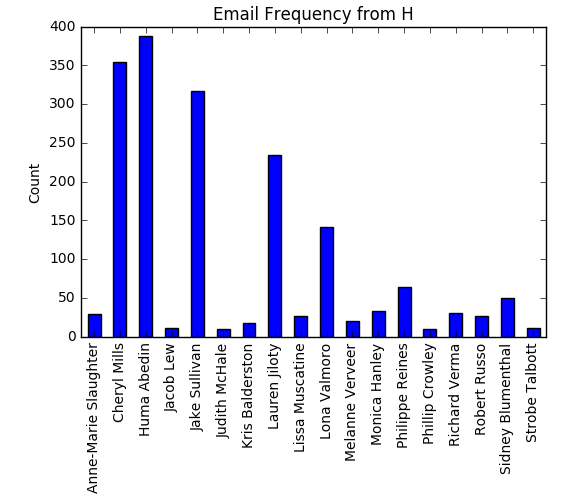
\includegraphics[scale=0.38]{pix/freq1.png}
}
\subfloat[Receiver is HC]{
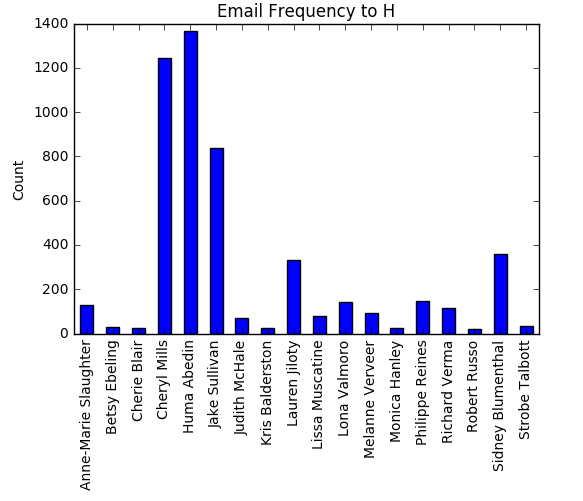
\includegraphics[scale=0.38]{pix/freq2.png}
}
\caption{Contact Frequency Profile}
\label{fig:contactf}
\end{figure}

\subsection{Topic Modelling}

In topic modelling, the observations are word collected into documents. Each topic is represented by some probability distribution over the vocabulary. Some words are most probable for a particular topic than the other. A document may belong to mixture of topics differently weigthed. Any topic modelling method assumes that the words that are similar in meaning will appear in similar pieces of text. We describe two kinds of topic model in the following.
\begin{itemize}
\item Latent Semantic Analysis: In this method a term doc matrix is formed where each row corresponds to a term or word and each column to a document. Each $(i,j)^{th}$ entry in the matrix represents number of occurence of term $i^{th}$ term in $j^{th}$ document. This method performs low rank approximation to the term doc matrix by SVD. The singular vectors correspond to the topics. Each topic can be seen as combination of component words weighted by their probability value.
\item Latent Dirichlet Allocation: Commonly known as LDA, this is a generative statistical model giving joint probability distribution for a topic-word combination. It is a problem of Bayesian inference where the objective is to learn several distribution parameters including the set of topics, their associated word probabilities, the topic of each word and the particular topic mixture of each document.
\end{itemize}

In our work, we have used Gensim's LDA as topic model. Each document(email body) has to be tokenized first. The tokens are used to create vocabulary. Then we represent each document as bag of such tokens or bag of words. BoW for the documents are normalized by tf-idf. Now the documents, in the form of normalized bag of words, are used to create LDA topic model.

In order to \textbf{evaluate} our model, we retrieve email-chains from the table by grouping emails by their subject(processed to contain original subject string). Our hope is that emails belonging to the same chain will more or less be of similar topic. We have picked email chains with more than ten emails and showed their contribution to several topics. In fig \ref{fig:topicd} the x-axis represents email chains in descending order of their email count. The stacked bar chart represent the topic proportion of each email. There are twenty topics T1 to T20 and marked with different colours. Each bar shows contribution to different topics of a particular email chain.

\begin{figure}
\center
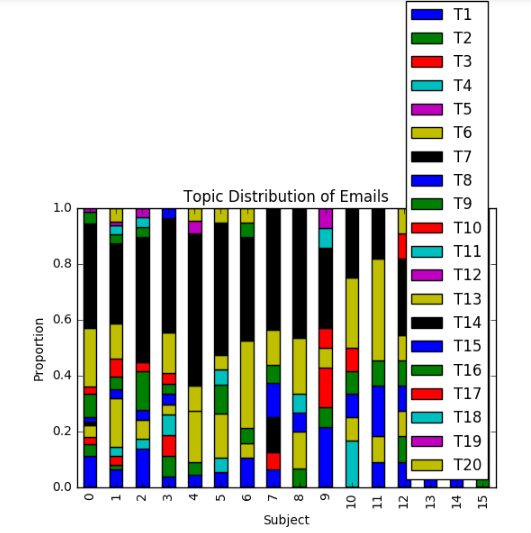
\includegraphics[scale=0.5]{pix/topic.png}
\caption{Topic distribution of email-chains}
\label{fig:topicd}
\end{figure}

\subsection{Sentiment Analysis}

Our objective was to identify overall binary(positive/negative) sentiment towards a nation by scanning all the email conversations. We have used VADER rule based model to assign positive, negative and neutral score to a sentence. This method does not just look at individual words to score a sentence, but it also considers the context. This pre-trained model comes with a lexicon file containing different terms each having some score for all three sentiments. Now the model has defined rules to predict sentiment for a sentence by combining its constituent words having their own scores. We find average positive/negative sentiment for a nation. We have used NLTK-VADER library for our purpose. Fig \ref{fig:nation_cnt} shows the number of times a nation has been mentioned in emails.

We present two ways of evaluating sentiment for a nation. One is document based while another is sentence specific. The methods are illustrated as follows:
\begin{itemize}
\item In document wise sentiment analysis, we compute average sentiment for each email text. Then for any country we find count of its mention over all emails. Now we compute sentiment for a country by sum of document sentiments weighted by the occurrence counts we have for the country in the emails. Figure \ref{fig:senti_doc} presents the result.
\item In sentence wise approach we only consider the sentences having mention about a country over entire email data. Sentiment for a nation is computed as average sentiment of all the relevant sentences we got. Figure \ref{fig:senti_sent} shows the result for positive and negative sentiments respectively.
\end{itemize}

We observed better results in the sentence wise approach. It is in hermony with the political trend in real time.

\begin{figure}[t!]
\center
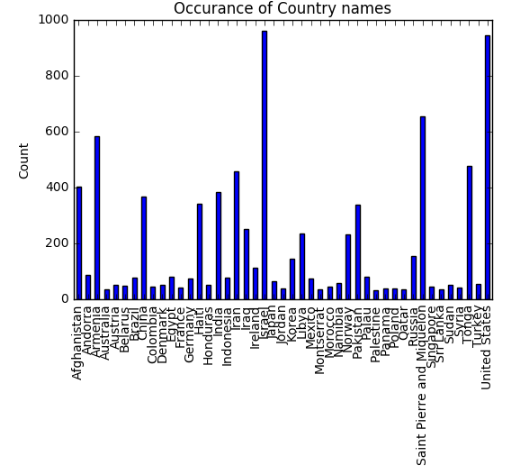
\includegraphics[scale=0.5]{pix/nation_cnt.png}
\caption{Occurrence of nation names}
\label{fig:nation_cnt}
\end{figure}

\begin{figure}
\subfloat[Postivity]{
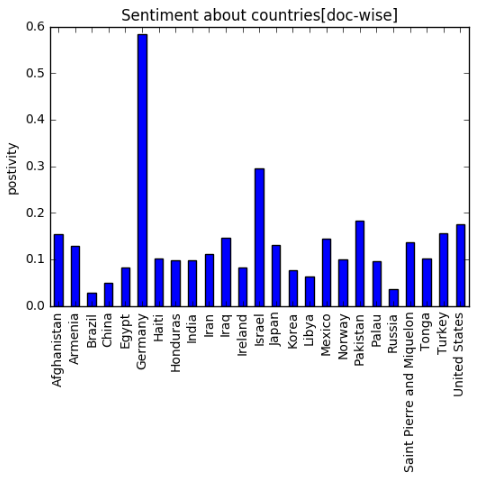
\includegraphics[scale=0.4]{pix/senti_pos_doc.png}
}
\subfloat[Negativity]{
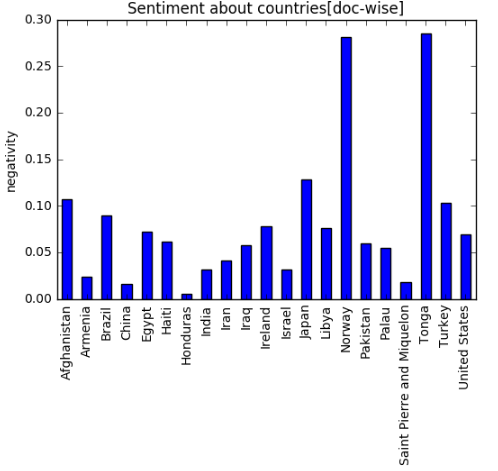
\includegraphics[scale=0.4]{pix/senti_neg_doc.png}
}
\caption{Document wise sentiment}
\label{fig:senti_doc}
\end{figure}

\begin{figure}[t!]
\subfloat[Postivity]{
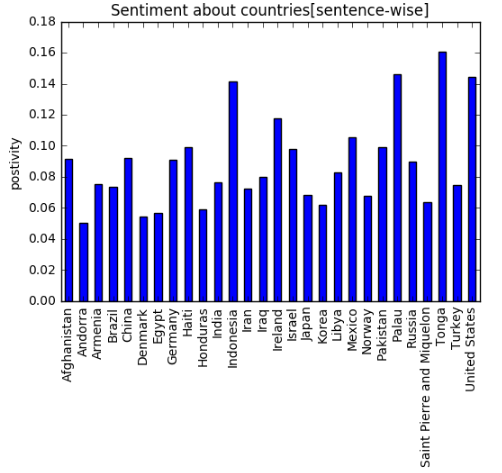
\includegraphics[scale=0.4]{pix/senti_pos_sent.png}
}
\subfloat[Negativity]{
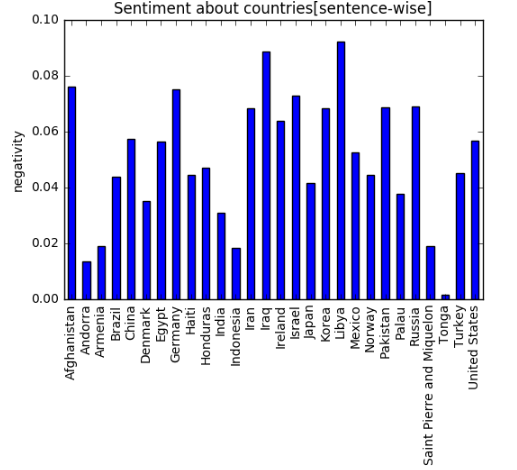
\includegraphics[scale=0.4]{pix/senti_neg_sent.png}
}
\caption{Sentence wise sentiment}
\label{fig:senti_sent}
\end{figure}

\section*{Learning and Conclusion}

In our work we have been able to quite fairly analyse the emails of US state secretary Hillary Clinton. We have consulted various forums including Kaggle discussion threads to know about the possible approach to solve a problem. We have also been helped by Gensim and NLTK documentations. For topic modelling we used pyLDAvis tool to generate a dynamic and interractive visualization showing relation among the topics in terms of cosine distance and the words incorporated in the topics. We did not include that in this static document. We learnt to use pandas in depth while playing with sql data.

Overall the project gave us a new exposure to modern techniques and tools used for Natural Language Processing.

\subsubsection*{References}
% may use bixtex to automatically generate the list of references or
% enter these manually below

\small{
[1] Wikipedia - Latent Dirichlet allocation

[2] Wikipedia - Latent semantic analysis

[3] Hutto, Clayton J., and Eric Gilbert. "Vader: A parsimonious rule-based model for sentiment analysis of social media text." Eighth International AAAI Conference on Weblogs and Social Media. 2014.
}

\end{document}
